\section{Background}


\subsection{DVMS}

\subsubsection{Overview.}
DVMS~\cite{quesnel:ispa13,quesnel:cpe12}
(Distributed Virtual Machine Scheduler) is a framework that can schedule VMs
cooperatively and dynamically in large scale distributed
systems.

DVMS is deployed as a set of agents that are organized following a ring
topology and that cooperate with one another to guarantee the quality of
service~(QoS) for the VMs.

When a node cannot guarantee the QoS for its hosted VMs or when it is
under-utilized, it starts an iterative scheduling procedure~(ISP) by querying
its neighbor to find a better placement; it thus becomes the initiator of the ISP.
If the request cannot be satisfied by the neighbor, it is forwarded to the
following free one until the ISP succeeds.

\subsubsection{Strengths.}
This approach allows each ISP to send requests only to a minimal
number of nodes, thus decreasing the scheduling time without requiring a
central point.
%
It is worth noting that an ISP can reserve all nodes of the
infrastructure if needed, i.e. if the corresponding problem is particularly hard to solve, thus
guaranteeing that a solution will always be found if it exists.

In addition, this approach allows several ISPs to occur independently at the
same moment throughout the infrastructure; in other words, scheduling is
performed on partitions of the system that are created dynamically, which
significantly improves the reactivity of the system.

Communications are handled efficiently, as each node involved in a partition
can forward a request directly to the first node outside its partition, by
means of a ``first out'' relation.

An example involving three partitions is shown on Figure~\ref{fig:isp}; in
particular, we can see the growth of partition~1 between two steps.
\begin{figure}[h!]
  \centering
  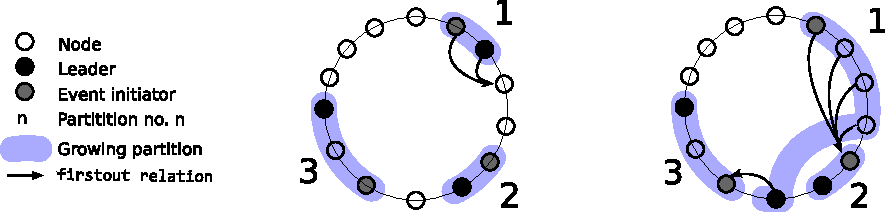
\includegraphics[width=0.9\linewidth]{Figures/resourceAcquisition-standard.pdf}
  \caption{Solving three problems simultaneously and independently with DVMS}%
  \label{fig:isp}%
\end{figure}

It is worth noting that (i)~the correctness of DVMS was proven
formally~\cite{quesnel:ispa13} and that (ii)~the first version of the prototype
was validated at large scale (up to 4.7k VMs and 470 nodes) by means of experiments on the Grid'5000
testbed~\cite{quesnel:ispa13},
and at very large scale (up to 80k VMs and 8k nodes) by means of simulations
with the SimGrid toolkit~\cite{Casanova:2008:SGF:1397760.1398183}.

\subsubsection{Limitations of the First Implementation.}

This first implementation of DVMS has several limitations; in this section, we
will focus on locality management.

Even if DVMS can be deployed across several sites, it performs better on a
cluster.
%
The reasons are simple.
%
First, the ring is built without taking account of the network topology;
therefore, a VM migration can occur between two nodes that are far from each
other, which lasts longer than a migration between two close nodes.
%
Second, even if the ring was built so that nodes with a fast interconnection
were close from one another, it would not prevent a node to communicate with 
a remote neighbor instead of a close one.

To sum up, the ring topology is far from ideal when considering locality
management, for instance in a multi-site deployment where we want to avoid
inefficient and costly inter-site VM migrations.

% Autres limitations :
% -absence de tolérance aux pannes
% -peu d'événements gérés (surcharge d'un noeud)
% -ne prend pas en compte les liens entre VMS



\subsection{P2P - locality}


La prise en compte de la localit? dans la construction de r?seaux logiques
(\emph{overlays}) a ?t? initialement propos? dans le r?seau logique structur?
Pastry~\cite{pastry} afin d'optimiser la latence du routage. La recherche de ces
n\oe uds proches est fond?e sur un ?change p?diodique de r?f?rences de n\oe uds.

Le m?me concept a ?t? propos? dans les r?seaux logiques non structur?s afin de
permettre ? chaque n\oe ud de d?couvrir des n\oe uds du syst?mes les plus
\emph{proches}. La notion de proximit? peut recouvrir toute m?trique transitive
entre deux n\oe uds, en particulier le temps de latence entre les n\oe
uds~\cite{refquivabienmarindoittrouver}.

Le protocole Vivaldi~\cite{dabek:2001:sigcomm04}, sur lequel notre r?seau logique est fond?,
a une approche particuli?re. En effet, il fournit ? chaque n\oe ud des
coordonn?es dans un espace multi-dimensionnel refl?tant sa position dans le
r?seau physique. Initialement, chaque n\oe ud prend une position al?atoire de
l'espace, et choisit un petit sous-ensemble de n\oe uds. Puis, il se rapproche
dans l'espace, des n\oe uds avec lesquels il a une faible latence et s'?loigne
dans le cas inverse. Vivaldi ne permet donc pas de conna?tre les n\oe uds qui
lui sont proches dans le r?seau, mais de les reconna?tre via leurs coordonn?es.

Les approches pr?c?dentes maintiennent constamment la connaissance des n\oe udes
proches afin de fournir le meilleur n\oe ud possible, au co?t de communications
p?riodiques (ind?pendamment de la quantit? de requ?tes effectives.) Notre
approche se distingue par une approche paresseuse consistant ? rechercher des
n\oe uds proches (en s'appuyant sur les coordonn?es Vivaldi) lors des requ?tes,
adaptant ainsi la qualit? de la r?ponse ? la fr?quence des requ?tes.

